\documentclass{article}
\usepackage[utf8]{inputenc}

\title{Tesina Distributed FS (main)}
\author{alessiocorrado99 }
\date{September 2020}

\usepackage{natbib}
\usepackage[utf8]{inputenc} %input chars
\usepackage[english]{babel} %language
\usepackage[T1]{fontenc} %output chars
\usepackage{lmodern} %font
\usepackage{geometry} %page layout
\usepackage{amsfonts} %math symbols
\usepackage{amsmath} %math equations
\usepackage{amssymb} %math symbols
\usepackage{mathtools} %other math
\usepackage{paralist} %lists
\usepackage{graphicx}
\usepackage{subcaption}
\usepackage{multirow}
\usepackage{verbatim}
\usepackage{multicol}
\usepackage{pgfplots} %plots
\usepackage{listings} %listings
\usepackage[outdir=./images]{epstopdf} %eps images
\usepackage{color} %colored text
\usepackage{algorithm2e}
\usepackage{float} %images going to end of the document
\usepackage{hyperref}
\makeatletter
\newcommand{\HEADER}[1]{\ALC@it\underline{\textsc{#1}}\begin{ALC@g}}
	\newcommand{\ENDHEADER}{\end{ALC@g}}
\makeatother
\usepackage{microtype} %better type
% questo sono i default per i listings 
\lstset{
	frame=tb, % draw a frame at the top and bottom of the code block
	tabsize=4, % tab space width
	showstringspaces=false, % don't mark spaces in strings
	breaklines=true,
	numbers=left, % display line numbers on the left
	basicstyle=\footnotesize,
	commentstyle=\color{green}, % comment color
	keywordstyle=\color{blue}, % keyword color
	stringstyle=\color{red} % string color
}

\DeclareRobustCommand{\univsc}[1]{\Large\textsc{\textls[75]{#1}}}
\DeclareRobustCommand{\titlesc}[1]{\linespread{1.2}\LARGE{\textls[35]{\uppercase{#1}}\linespread{1}}}
\DeclareRobustCommand{\namesc}[1]{\large\textsc{\textls[35]{#1}}} 

\newcommand{\facciatabianca}{\newpage\shipout\null}

\allowdisplaybreaks

\begin{document}

\maketitle

\section{Introduzione} 

\paragraph{} Lo scopo del progetto è la realizzazione di un \textbf{file storage distributito}. 

\paragraph{} Le caratteristiche che deve avere sono:

\begin{itemize}
	\item \emph{Efficienza}: I tempi di risposta devono essere ragionevoli e non degradare con l'aumento del numero di nodi. L'utilizzo delle risorse a disposizione deve essere massimizzato, ovvero non devono esserci risorse inutilizzate o carichi di lavori troppo sbilanciati.  
	
	\item \emph{Accesso concorrente}: Più client possono effettuare richieste in modo concorrente. Deve essere tenuta in considerazione qualche politica di \emph{fairness}, 
	in modo che nessun client sia privilegiato o venga escluso. Deve essere garantita la 
	\emph{consistenza} specificamente in caso di accessi concorrenti alla stessa risorsa. 
	 
	\item \emph{Replicazione dei dati (files)}: Per garantire un buon livello di \emph{fault tolerance}, tutti i dati devono essere replicati. In questo modo problematiche su un nodo non compromettono il contenuto di un file. 
	
	\item \emph{Replicazione dei metadati (struttura del fs)}: La struttura del \emph{file system} deve essere sempre replicata, in modo che non possa essere persa o corrotta a seguito di problemi. 
\end{itemize} 



\paragraph{Numero di repliche}

Il numero di repliche di un file deve essere \underline{proporzionale} sia all'importanza che al numero di accessi di esso: file con \emph{dati critici} hanno numero di copie maggiore, per agevolarne la \emph{disponibilità} e diminuire le \emph{probabilità di perdita}. 

Il \emph{numero di repliche minimo} è: 2.

\paragraph{Bilanciamento del carico} Per migliorare l'efficienza viene effettuato un bilanciamento del carico: in ogni momento i file vengono \underline{copiati} o \underline{spostati} in modo da non sovraccaricare un singolo nodo. Inoltre, per il trasferimento di un file si cerca di utilizzare il nodo con maggiore \emph{banda disponibile}. 



\section{Architettura del sistema}

Verranno di seguito analizzate diverse possibili architetture del sistema, comparandone pregi e difetti. 

\subsection{Single-server}

\paragraph{} La prima idea è quella di avere un \emph{singolo server}, il quale memorizza \emph{sia la struttura del fs che i dati}. Il client interagisce direttamente con esso per effettuare qualsiasi operazione. 

\paragraph{} Il fs può essere memorizzato a partire da una \emph{directory nel filesystem del server}, oppure in una \emph{partizione separata}. Con entrambe le soluzioni è il sistema operativo ad occuparsi della sua gestione.

\paragraph{} La \emph{replicazione dei dati} avviene mediante il salvataggio in \underline{diversi dispositivi di memorizzazione} (es HDD). Per far ciò la scelta più consona è di utilizzare un sistema \textbf{RAID 10}: i dati vengono \underline{salvati in copia} (RAID 1) per avere \emph{tolleranza ai guasti} e in \underline{striping} (RAID 0) per aumentare la \emph{velocità di lettura}. 

\paragraph{} Con \underline{schede di rete (e connessioni) multiple} è possibile migliorare la tolleranza sia ai \emph{guasti} che alle \emph{congestioni di rete}. 

\paragraph{Vantaggi} \begin{itemize}
	\item Semplice da implementare
	\item Modello più economico
	\item Il fs è gestito direttamente dal sistema operativo
	\item Minima esposizione contro attacchi hacker
	\item Con gli accorgimenti sopra descritti si ha già una buona fault tolerance. 
\end{itemize} 

\paragraph{Svantaggi} \begin{itemize}
	\item \emph{Single point of failure} per quanto riguarda il server (i dati sono parzialmente protetti dal meccanismo RAID)
	\item Nessuna protezione per \emph{eventi eccezionali} (eg. catastrofe naturale, incendio nell'edificio, blocco della rete\dots). 
\end{itemize}. 

\begin{figure}[H]
	\centering
	\begin{subfigure}{0.60\linewidth}
		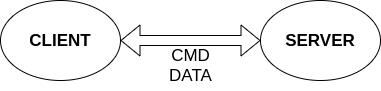
\includegraphics[width=\linewidth]{../diagrams/architettura/1.png}
	\end{subfigure}
	\caption{Single-server}
\end{figure}



\subsection{Virtual server}

\paragraph{} La soluzione single-server può essere migliorata aggiungendo un \emph{livello di virtualizzazione}. Il sistema operativo non viene quindi eseguito direttamente sull'hardware ma all'interno di un \underline{container/VM}. 

\paragraph{} La macchina virtuale viene periodicamente \emph{copiata} (interamente o in modo incrementale) e salvata in un \underline{dispositivo di memorizzazione dedicato}. 

\paragraph{} Nel caso ci fosse un \emph{crash} o \emph{errore critico del sistema operativo}, basta ricaricare la macchina virtuale più recente. La \emph{perdita di dati} è limitata all'età dell'ultimo backup. 

\paragraph{Vantaggi} \begin{itemize}
	\item \emph{Recovery} buona e in tempi brevi in caso di crash. 
\end{itemize}


\paragraph{Svantaggi} \begin{itemize}
	\item Durante il \emph{periodo di transizione} il sistema non risponde
	\item \emph{Prestazioni} leggermente ridotte a causa della virtualizzazione
\end{itemize}

\begin{figure}[H]
	\centering
	\begin{subfigure}{0.60\linewidth}
		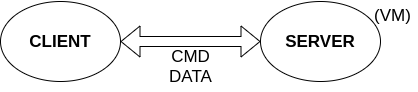
\includegraphics[width=\linewidth]{../diagrams/architettura/2.png}
	\end{subfigure}
	\caption{Single-server con virtualizzazione}
\end{figure}



\subsection{Cloud backup}

\paragraph{} Il backup può essere effettuato nel \underline{cloud}, al posto che in un dispositivo dedicato all'interno del datacenter. Inoltre il backup può essere esteso anche ai dati, oltre che al fs. 

\paragraph{Vantaggi} \begin{itemize}
	\item Protezione in caso di \emph{eventi eccezionali}
\end{itemize}

\paragraph{Svantaggi} \begin{itemize}
	\item In generale effettuare un backup nel cloud, anche se solo incrementale, richiede un \emph{elevato utilizzo di banda} e \emph{tempi maggiori} 
	\item \emph{Costi} maggiori 
\end{itemize}

\begin{figure}[H]
	\centering
	\begin{subfigure}{0.80\linewidth}
		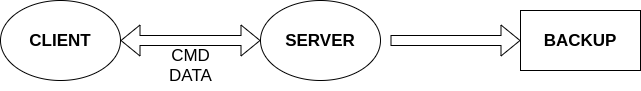
\includegraphics[width=\linewidth]{../diagrams/architettura/3.png}
	\end{subfigure}
	\caption{Aggiunta del backup nel cloud}
\end{figure}



\subsection{Server as distributed database}

\paragraph{} Al posto di utilizzare il file system del sistema operativo, è possibile utilizzare un \underline{database distribuito}. Sia metadati che dati vengono \emph{distribuiti automaticamente} nei nodi, garantendo consistenza e fault tolerance. 


\paragraph{Vantaggi} \begin{itemize}
	\item I dati vengono automaticamente replicati e gestiti dal dbms
	\item Utilizzando un dbms in commercio, si beneficia dall'avere tutto già pronto e costantemente aggiornato.
\end{itemize}


\paragraph{Svantaggi} \begin{itemize}
	\item Maggiore complessità
	\item La connessione avviene tra il client ed un nodo, il quale poi distribuisce i dati agli altri nodi. Se questo nodo dispone di una banda limitata, ciò può rappresentare un bottleneck dal punto di vista delle prestazioni. 
\end{itemize}

\begin{figure}[H]
	\centering
	\begin{subfigure}{0.80\linewidth}
		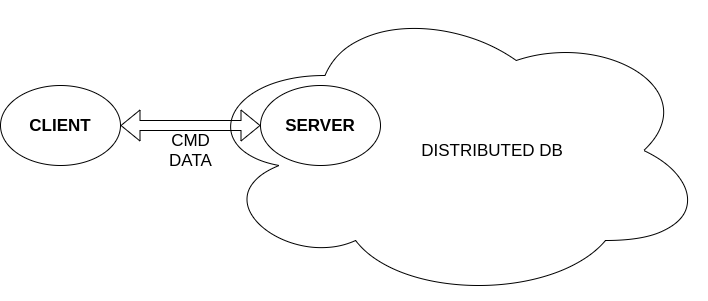
\includegraphics[width=\linewidth]{../diagrams/architettura/4.png}
	\end{subfigure}
	\caption{Utilizzo di un database distribuito}
\end{figure}



\subsection{Meta+Data server}

\paragraph{} L'idea è di far \emph{comunicare direttamente il client con i server in cui verranno memorizzati i dati}. Così facendo si elimina il bottleneck del nodo che prima doveva fungere da "gateway". 

\paragraph{} Un primo sviluppo è quello di \emph{separare i compiti}: si hanno quindi \underline{un} \textbf{meta server} e \underline{uno o più} \textbf{data server}. Il meta server si occupa di memorizzare e gestire il file system (metadati), mentre i data server memorizzano soltanto i dati conenuti nei file. 

\paragraph{} Per effettuare una qualsiasi \emph{operazione di trasferimento} il client si rivolge inizialmente al meta server, dal quale ottiene la configurazione per contattare il giusto data server e trasferire i dati. Le \emph{operazioni sul filesystem} sono eseguite all'interno del meta server. In questo modo ci sono \emph{due comunicazioni bidirezionali}: client-meta, per la gestione del fs; client-data, per il trasferimento dei dati.

\paragraph{} Per migliorare le prestazioni, soprattutto nel caso in cui il client abbia una banda più ampia rispetto ai data server, i file di grandi dimensioni vengono spezzati in \underline{chunks} e distribuiti. 

\paragraph{} Come nel caso single-sever, il meta server è unico, virtualizzato e sottoposto a backup periodico. 

\paragraph{Vantaggi} \begin{itemize}
	\item Trasferimenti concorrenti con data server multipli permettono di migliorare le prestazioni nel caso in cui il client abbia una banda elevata
	\item Un \emph{unico meta server} permette di mantenere in modo semplice la consistenza del file system
\end{itemize}

\paragraph{Svantaggi} \begin{itemize}
	\item La frequenza dei \emph{backup} del meta server è fondamentale per minimizzare la perdita di dati in caso di fault
	\item Tutti i data server devono essere \emph{raggiungibili} dal client (maggiore attenzione alla sicurezza e struttura della rete)
\end{itemize}

\begin{figure}[H]
	\centering
	\begin{subfigure}{0.60\linewidth}
		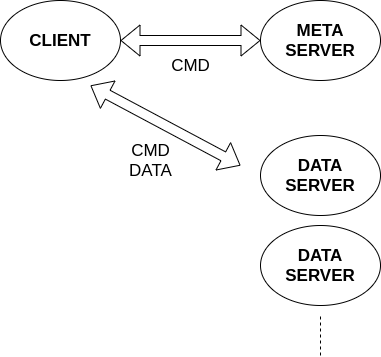
\includegraphics[width=\linewidth]{../diagrams/architettura/5.png}
	\end{subfigure}
	\caption{Separazione di meta e data server}
\end{figure}



\subsection{Meta+Data server 2}

\paragraph{} Facendo dialogare meta e data server, è possibile:\begin{enumerate}
	\item Spostare l'\emph{onere di configurazione dei data server} da client a meta server
	\item Gestire in qualsiasi momento la \emph{replicazione dei dati}, esempio per bilanciare il carico o far fronte alla perdita di un nodo
	\item Il meta server può monitorare \emph{prestazioni} e \emph{stato di salute} dei data sever
\end{enumerate}

\paragraph{} Il client quindi si limita a trasferire i dati da/verso data server utilizzando \underline{token} forniti dal meta server. 

\paragraph{Vantaggi} \begin{itemize}
	\item Il sistema può \emph{riconfigurarsi} in ogni momento per far fronte a qualsiasi evenienza
	\item Ruolo del client semplificato 
	\item Maggiore sicurezza (minore esposizione) perchè il client non può inviare comandi ai data server
\end{itemize}


\paragraph{Svantaggi} \begin{itemize}
	\item Maggiore complessita nel gestire operazioni \emph{concorrenti} ed \emph{asincrone} in nodi diversi
\end{itemize}

\begin{figure}[H]
	\centering
	\begin{subfigure}{0.60\linewidth}
		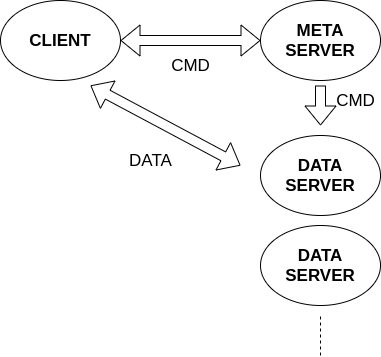
\includegraphics[width=\linewidth]{../diagrams/architettura/6.png}
	\end{subfigure}
	\caption{Meta + data server, il meta server dialoga con i data server}
\end{figure}



\subsection{Meta server as distributed system}

\paragraph{} In questa soluzione non è presente un unico meta server, ma viene utilizzato un sistema distribuito. In generale è preferibile utilizzare un dbms distribuito presente in commercio.

\paragraph{} Come dimostrato dal teorema CAP bisogna rinunciare alla disponibilità per garantire la coerenza del fs. 

\paragraph{Vantaggi} \begin{itemize}
	\item Possibilità di utilizzo di software in commercio
	\item Maggiore fault tolerance dei metadati
	\item Minore tempo di down in caso di malfunzionamenti
\end{itemize}

\paragraph{Svantaggi} \begin{itemize}
	\item Maggiore difficoltà nell'implementazione dei meta server e dei protocolli di comunicazione tra i vari componenti. 
	\item Maggiore overhead (e quindi minori prestazioni) nel caso di sistemi di piccole/medie dimensioni
\end{itemize}

\begin{figure}[H]
	\centering
	\begin{subfigure}{0.80\linewidth}
		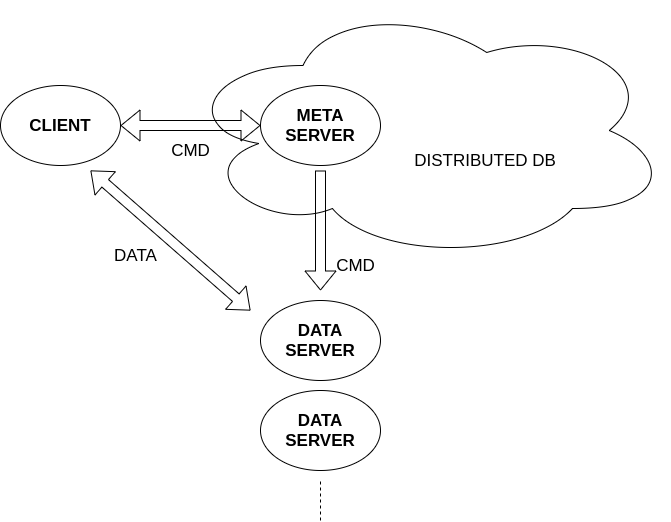
\includegraphics[width=\linewidth]{../diagrams/architettura/7.png}
	\end{subfigure}
	\caption{Il meta server è implementato come database distribuito}
\end{figure}



\section{Comandi del client}

Di seguito l'elenco e descrizione dei comandi gestiti dal client.

\begin{itemize}
	\item list(path="root", recursive=true, inclue\_meta=false, format=json)
	
	Lista il contenuto di una cartella.
	
	Argomenti: \begin{itemize}
		\item path: directory target. Default: "root"
		\item recursive: solo cartella o tutto il sottoalbero. In ogni caso non segue i link. Default: true
		\item include\_meta: include i metadati relativi ad ogni entry. Default: false
		\item format: formato di output. valori: csv, json. Default: json.
	\end{itemize}
	
	\item mkdir(path)
	
	Crea una directory
	
	\item meta(path)
	
	Metadati di un path
	
	\item get(path)
	
	Download di un file
	
	\item push(file, path) 
	
	Upload di un file
	
	\item rem(path)
	
	Delete di un path 
\end{itemize}




\section{Metadati dei path}

I metadati associati ad un path sono: 

\begin{enumerate}
	\item uid: identificatore univoco dell'oggetto
	\item path
	\item creation\_date
	\item size: dimensione in byte, 0 per le directory
	\item owner: utente proprietario, default chi l'ha creato
	\item visible: true/false. Indica se è visibile agli utenti diversi dall'owner
	\item min\_copies: numero minimo di copie, coincide con la priorità 
\end{enumerate}


\section{Protocollo comunicazione}

Di seguito i flussi di dati coinvolti nelle diverse tipologie di richieste.

\subsection{get}

\paragraph{} La richiesta di tipo \emph{get(path)} richiede il trasferimento in entrata di un file. 

\paragraph{} Inizialmente il \emph{client} contatta il \emph{meta server}, richiedendo un particolare \emph{path}. Il \emph{meta server} seleziona il \emph{data server} ottimale per gestire la richiesta (deve contenere la risorsa e non essere sovraccarico). Il \emph{meta server} risponde quindi al client specificando l'uid della risorsa (richiesto per identificarla) e l'indirizzo del \emph{data server} a cui collegarsi. Il \emph{client} si disconnette dal \emph{meta server}.

\paragraph{} Il \emph{client} si connette al \emph{data server} inviando una richiesta \emph{get(uid,start\_pos)}. L'argomento \emph{start\_pos} indica da che byte iniziare a trasferire il file (indice 0-based). Se la risorsa è disponibile (come dovrebbe essere) il \emph{data server} invia un \emph{ack} seguito dal flusso di dati del file.) Altrimenti risponde con \emph{err} seguito dai dettagli. 

\begin{figure}[H]
	\centering
	\begin{subfigure}{0.80\linewidth}
		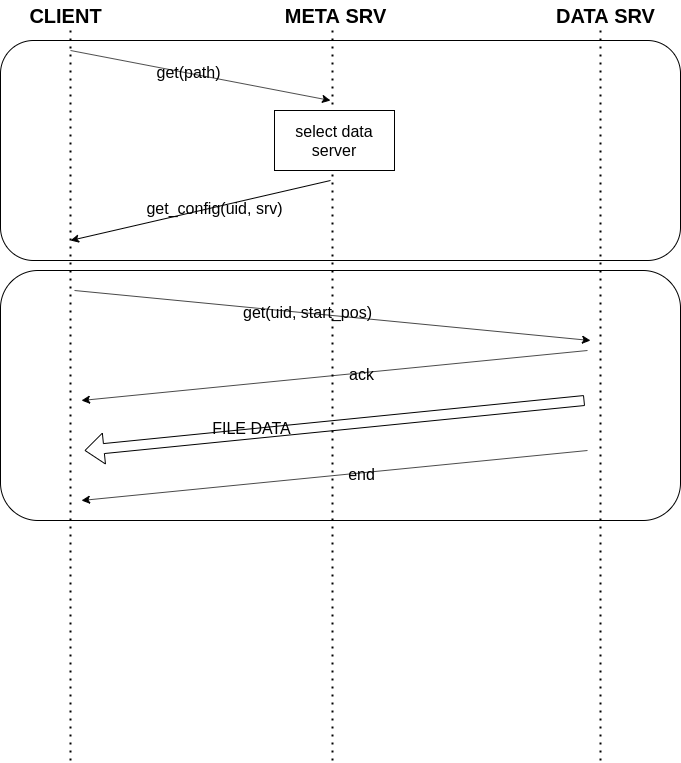
\includegraphics[width=\linewidth]{../diagrams/requests/get_request.png}
	\end{subfigure}
\end{figure}


\subsection{push}

\paragraph{} La richiesta di tipo \emph{push(path, data)} richiede il trasferimento in uscita di un file da parte del client. 

\paragraph{} Inizialmente il \emph{client} contatta il \emph{meta server}, inviando \emph{path} e \emph{size}. Il \emph{meta server} seleziona il \emph{data server} ottimale per gestire la richiesta (deve poter contenere la risorsa e non essere sovraccarico). Il \emph{meta server} si occupa anche di generare un nuovo \emph{uid} da assegnare alla risorsa. 

\paragraph{} Il \emph{meta server} si collega al \emph{data server} dove verrà inizialmente salvata la risorsa, inviando un comando \emph{create(uid, size)}. Questo comando predispone il \emph{data server} per ospitare un nuovo documento con tale uid e dimensione. Se non ci sono errori, il \emph{data server} risponde al \emph{meta server} con \emph{ack}. Altrimenti con \emph{err} seguito dai dettagli.

\paragraph{} Il \emph{meta server} risponde quindi al client specificando l'uid della risorsa (richiesto per identificarla) e l'indirizzo del \emph{data server} a cui collegarsi. Il \emph{meta server} si disconnette dal \emph{client} e invia le eventuali richieste di eliminazione ai data server (se il file è una nuova versione di uno esistente).

\paragraph{} Inizia quindi il caricamento del documento. Il \emph{client} si collega al \emph{data server} e invia una \emph{push(uid)}. Se non ci sono errori, il \emph{data server} risponde con \emph{ack} e invia la posizione (indice 0-based) \emph{last\_pos} del primo byte non trasferito (equivalente al numero di byte già trasferiti). A quel punto il \emph{client} trasferisce la porzione rimanente di documento. Al termine del trasferimento, se non ci sono errori, il \emph{data server} risponde con \emph{ack}. La connessione viene chiusa.

\paragraph{} Quando il trasferimento è completato con successo, inizia la terza fase. Il \emph{data server} invia un messaggio del tipo \emph{push\_complete(uid)} al \emph{meta server}. Il meta server inizia quindi ad inviare ai \emph{data server} interessati le richieste di trasferimento, per raggiungere il grado di replicazione voluto.

\begin{figure}[H]
	\centering
	\begin{subfigure}{0.80\linewidth}
		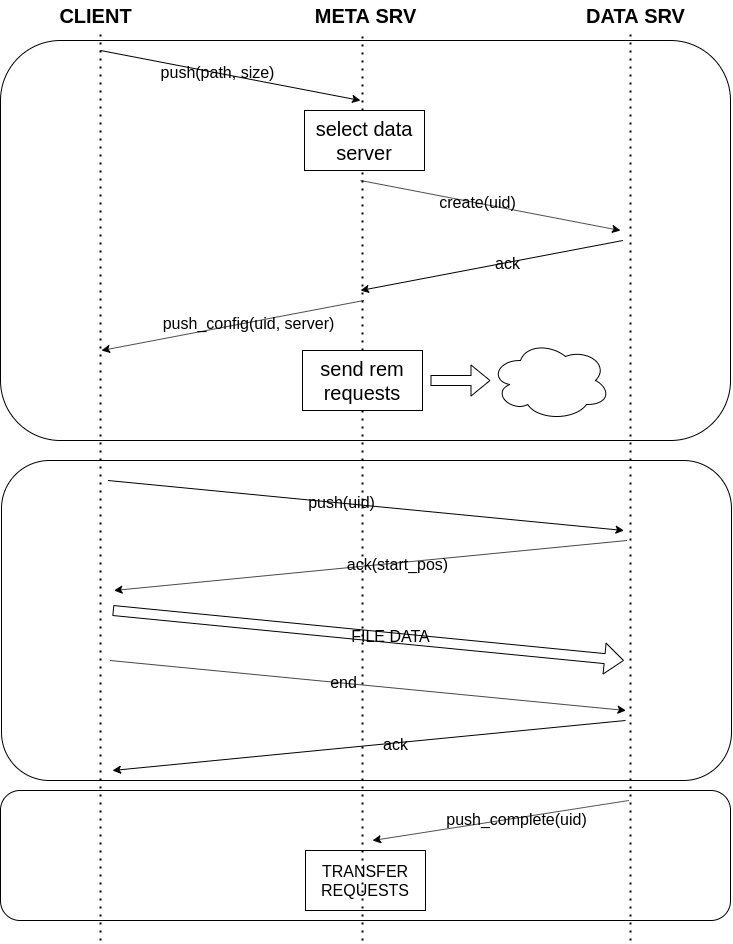
\includegraphics[width=\linewidth]{../diagrams/requests/push_request.png}
	\end{subfigure}
\end{figure}


\subsection{rem}

\paragraph{} La richiesta di tipo \emph{rem(path)} richiede l'eliminazione di un file/directory dallo storage.

\paragraph{} Il \emph{client} invia al \emph{meta server} una richiesta \emph{rem(path)}. Se non ci sono errori, il \emph{meta server} risponde con \emph{ack} e chiude la connessione.

\paragraph{} Il \emph{meta server} contatta separatamente tutti i \emph{data server} contenenti dati relativi a quel particolare \emph{uid} e invia una richiesta \emph{rem(uid)}.  

\begin{figure}[H]
	\centering
	\begin{subfigure}{0.80\linewidth}
		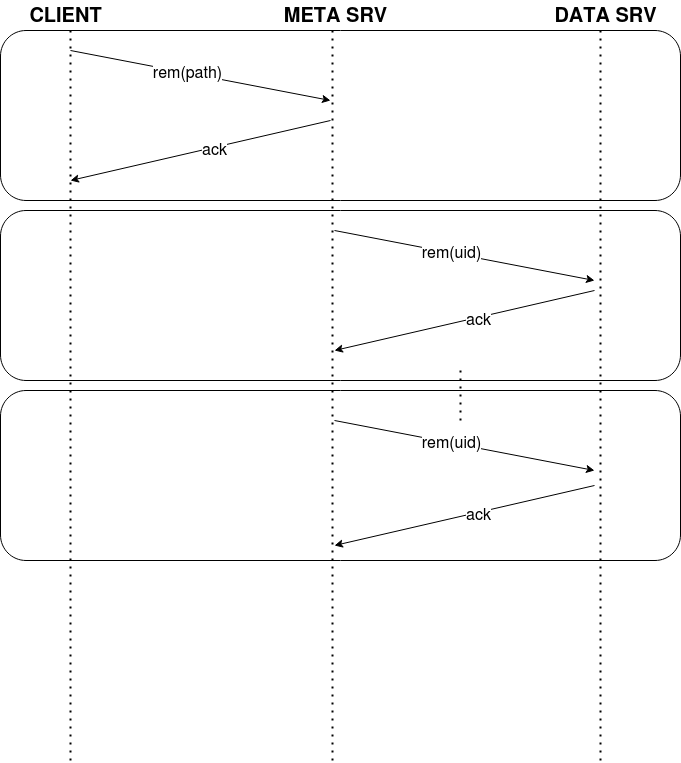
\includegraphics[width=\linewidth]{../diagrams/requests/rem_request.png}
	\end{subfigure}
\end{figure}



\subsection{transfer}

\paragraph{} La richiesta di tipo \emph{transfer} richiede la copia di un file (uid) da un \emph{data server} ad un altro. Viene usata dal \emph{meta server} per trasferire i dati tra i nodi e gestire la ridondanza.

\paragraph{} Inizialmente, come nel caso di una \emph{push}, il meta server contatta il \emph{data server} di destinazione (\emph{DATA2}) tramite una richiesta \emph{create(uid)}, per inizializzarlo a ricevere il file. Se non ci sono errori il \emph{data server} risponde con \emph{ack}. La connessione viene chiusa. 

\paragraph{} A questo punto il \emph{meta server} invia al \emph{data server} di origine (\emph{DATA1}) una richiesta \emph{transfer(uid, to)} per ordinare il trasferimento. Se \emph{DATA1} riesce a connettersi con successo a \emph{DATA2}, risponde a \emph{META} con \emph{begin\_transfer(uid)}. \emph{META1} invia a \emph{META2} una richiesta di tipo \emph{push(uid)} e da luogo al trasferimento. Al termine \emph{DATA1} invia un messaggio \emph{end\_transfer(uid)} a \emph{META} per notificare l'avvenuto trasferimento.


\begin{figure}[H]
	\centering
	\begin{subfigure}{0.80\linewidth}
		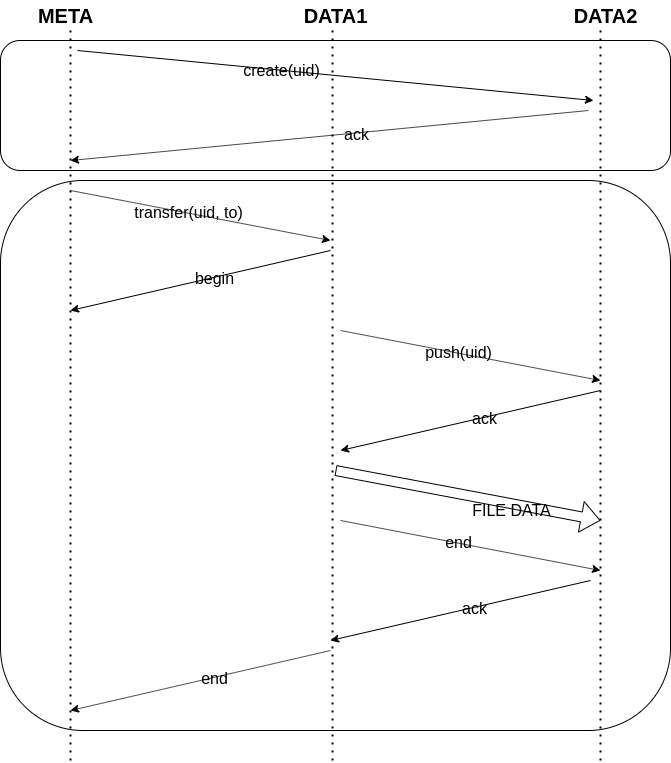
\includegraphics[width=\linewidth]{../diagrams/requests/transfer_request.png}
	\end{subfigure}
\end{figure}




\section{Logging}

\paragraph{} Tutte le operazioni prima di essere eseguite vengono registrate in appositi database di log. In questo modo, se un'operazione viene interrotta per qualsiasi motivo, può essere analizzata e rieseguita, in modo da non lasciare spazzatura. 





\section{Sicurezza ed autenticazione}

\paragraph{} Tutte le connessioni vengono cifrate tramite protocollo TLS over TCP. In questo modo la cifratura è invisibile alla logica dell'application e può in ogni momento essere modificata dal programmatore. Inoltre, essendo una tecnologia ampiamente diffusa e collaudata, presenta una vulnerabilità minima. 

\paragraph{} L'autenticazione da client a server avviene tramite coppia \emph{(username, password)} all'inizio della connessione. La password di ciascun utente può essere cambiata in ogni momento dall'utente stesso, dopo essersi loggato. 

\paragraph{} L'autenticazione da server a server avviene tramite certificato digitale. 




\bibliographystyle{plain}
\bibliography{references}
\end{document}
